\documentclass[pdflatex,sn-mathphys-num]{sn-jnl}

\usepackage[utf8]{inputenc}
\usepackage[T1]{fontenc}
\usepackage{graphicx}
\graphicspath{{../}}
\usepackage{multirow}
\usepackage{amsmath,amssymb,amsfonts}
\usepackage{amsthm}
\usepackage{mathrsfs}
\usepackage[title]{appendix}
\usepackage{xcolor}
\usepackage{textcomp}
\usepackage{manyfoot}
\usepackage{booktabs}
\usepackage{array}
\usepackage{url}

\newcommand{\pir}{\mathrm{PIR}}
\newcommand{\rmpir}{\mathrm{RM\text{-}PIR}}

% The bundled Springer Nature class stores the abstract through a command.
% This adapter preserves that machinery while allowing the requested
% \begin{abstract} ... \end{abstract} source syntax.
\let\snabstract\abstract
\let\abstract\relax
\let\endabstract\relax
\NewDocumentEnvironment{abstract}{+b}{\globaldefs=1\snabstract{#1}}{}

\raggedbottom

\begin{document}

\title[RM-PIR and team-ledger concordance]{RMS-matched Performance Index Rating improves EuroLeague team-ledger concordance with game outcomes}

\author*[1]{\fnm{[First name]} \sur{[Family name]}}\email{[corresponding.author@institution.example]}
\author[1]{\fnm{[First name]} \sur{[Family name]}}
\author[1]{\fnm{[First name]} \sur{[Family name]}}
\affil*[1]{\orgdiv{[Department]}, \orgname{[Institution]}, \orgaddress{\city{[City]}, \postcode{[Postcode]}, \country{[Country]}}}

\begin{abstract}
EuroLeague Performance Index Rating (PIR) is an additive box-score ledger with unit weights, and its team total can rank the losing team above the winner. We evaluated RMS-matched PIR (RM-PIR), a season-locked recalibration that fixes the point coefficient at one, estimates bounded nonpoint weights from no more than three completed prior seasons, and matches the calibration-sample root mean square (RMS) of official nonpoint winner--loser contrasts. The primary operational outcome was complete-score winner--loser ordering; nonpoint ordering was the mechanism analysis. Across five rolling historical target seasons (1,690 games), complete-score discordances decreased from 150 under official PIR to 104 under RM-PIR. In 2025--26 (402 games), they decreased from 27 to 21 (paired difference, -1.49 percentage points; game-bootstrap 95\% interval, -3.23 to 0.25), whereas nonpoint discordances decreased from 68 to 45 (-5.72 percentage points; -8.46 to -2.99). RM-PIR retained an auditable additive team ledger, including explicit accounting for team-only events. The findings are retrospective and criterion-specific: they support improved team-ledger concordance in these backtests, not causal player impact or validated individual player credit.
\end{abstract}

\keywords{EuroLeague, basketball analytics, performance index rating, box-score metrics, outcome concordance, rolling-origin backtest, RMS matching}

\maketitle

\section{Introduction}

Professional basketball is simultaneously an elite competition, a labour market, a media property and a large-scale entertainment product. The economic setting in which EuroLeague performance is evaluated is therefore substantial. A 2026 valuation prepared by JB Capital and released by Euroleague Basketball estimated the combined enterprise value of the competition and its licensed clubs at more than \(\mathrm{EUR}\,3.2\) billion, comprising \(\mathrm{EUR}\,1.41\) billion for the league and approximately \(\mathrm{EUR}\,1.8\) billion for licensed clubs \cite{EuroleagueValuation2026}. Enterprise value is not equivalent to annual revenue, but it indicates the scale of the assets, contracts and strategic decisions associated with the competition. The link between commercial capacity and sporting expenditure is also embedded in league governance: the EuroLeague Competitive Balance Standards connect club revenues to player-remuneration thresholds and establish a base net remuneration level of \(\mathrm{EUR}\,10\) million for the 2025--26 season \cite{EuroleagueCBS2025}. In this environment, the quality of performance measurement is not merely a statistical concern; it also shapes how clubs interpret the sporting return from high-value roster investments.

Clubs allocate finite resources across player recruitment, contract renewal, transfers and buyouts, coaching, medical support, player development and analytics. Quantitative analysis is now used in professional basketball to inform team strategy, player health management and personnel decisions, while investment in analytics has been associated with improved team-level performance in the NBA \cite{TernerFranks2021,WangSarkerHosoi2025}. EuroLeague-specific research likewise emphasises the practical relevance of objective player profiles for scouting, recruitment and roster construction \cite{PaulauskasEtAl2024}. Clubs' proprietary decision systems are not publicly observable, and no responsible investment decision should be reduced to one statistic. Nevertheless, a transparent performance index provides a common descriptive layer for post-game review, longitudinal monitoring, comparison of players in similar roles and evaluation of the team as a whole. Because PIR is additive, the credits and penalties assigned to player actions are aggregated in a team ledger. This structure makes PIR especially attractive for examining both individual production and the realised collective output of a roster, provided that the underlying action weights are defensible.

The same index also affects the public interpretation of EuroLeague basketball. Euroleague Basketball reported that the 2025--26 regular season generated a cumulative audience of 508.17 million across live, delayed and highlights formats, 1.49 billion video views on league-owned social-media platforms and a record 3,251,706 in-arena spectators \cite{EuroleagueEngagement2026}. At this scale, statistics are part of the entertainment product: they organise post-game discussion, support comparisons, create historical records and give fans a concise account of why a performance mattered. PIR has direct institutional salience because the EuroLeague MVP of the Round is awarded to the player with the highest PIR among players whose teams won \cite{EuroleagueAwards2024}. The explicit winning-team condition is important: it already recognises that individual box-score production must be interpreted in relation to the team outcome.

Performance indicators compress multidimensional sporting activity into quantities that can be compared across games, teams and seasons. Their usefulness depends on a clearly defined purpose, stable recording conventions and an explicit account of what is omitted \cite{HughesBartlett2002,MandicEtAl2019}. Media reporting necessarily compresses a complex game into a limited number of accessible narratives. A single index is valuable precisely because it can be communicated immediately and reconstructed from an official box score. Its limitation is not a failure of reporting, but a consequence of treating a multidimensional performance as one scalar quantity. Conventional box-score indices do not fully observe off-ball spacing, screen creation, defensive positioning, matchup difficulty, shot deterrence, lineup interaction or the leverage of an action at a particular game state \cite{DeshpandeJensen2016,SarlisTjortjis2020,TernerFranks2021,reich2006,franks2015,cervone2016,gudmundsson2017,jiao2021}. A reporting gap can arise when a partial index is read as a complete estimate of player impact. The gap is more consequential when the index's arithmetic assigns a larger team total to the losing team, because the same formula then distributes player credit in a way that is less consistent with the completed-game result. A more outcome-concordant primary index cannot eliminate the need for video, lineup and contextual analysis, but it can reduce this inconsistency at the source.

Official EuroLeague PIR has a major practical advantage: it is transparent and can be reconstructed from the competition's standardised team and player box-score fields \cite{EuroleagueStatsManual2025,KamitsisPolitis2025}. It awards one unit for points, rebounds, assists, steals, blocks and fouls drawn, and subtracts one unit for missed field goals, missed free throws, turnovers, blocks against and fouls committed. Additivity permits the same formula to be evaluated on player and team rows and makes every weighting assumption visible. Equal unit weights, however, implicitly treat heterogeneous events as equivalent units of credit or cost. The broader basketball-analytics literature has long emphasised possession-based comparison and the need to relate recorded actions to team success \cite{Oliver2004,KubatkoEtAl2007}. EuroLeague and related elite-basketball evidence shows that shooting efficiency, rebounding, assists, steals, turnovers and fouling have different relationships with winning, and that those relationships vary with competitive stage, game context, sex and competition level \cite{Ozmen2016,Cene2018,MikolajecEtAl2021,CharamisEtAl2023,SansoneEtAl2024,IbanezEtAl2008,CabarkapaEtAl2022}. Equal unit weights are therefore an auditable convention rather than an empirically calibrated statement that every recorded action contributes equally to the completed-game ledger.

For an additive post-game index, we selected the proportion of completed games in which the winning team's total exceeds the losing team's total as the team-level estimand. This is a normative outcome-concordance criterion, not an objective error definition: PIR can also be read as box-score production without requiring it to reproduce the winner. Nor does the criterion imply that every valuable individual performance must occur in a victory or that a box-score rating measures a player's causal effect. Because points define the winner, the complete-score criterion is mechanically related to the outcome. A points-only score would be perfectly concordant while discarding rebounds, assists, steals, blocks, fouls, missed shots and turnovers. The nonpoint analysis is therefore the key mechanism check: it tests the learned relative action direction apart from the direct point-margin contribution.

An apparent alternative would be to replace EuroLeague PIR with a metric developed for the National Basketball Association. This is not methodologically equivalent. The NBA and NBA-domain metric ecosystem comprises measures with different estimands and data requirements, rather than a single direct counterpart to EuroLeague PIR. For example, the NBA's Player Impact Estimate expresses a player's statistical production as a proportion of the total statistical production in the game, whereas plus-minus and Net Rating describe the score differential while a player is on court \cite{NBAStatsGlossary2026}. Regularised adjusted plus-minus models use lineup or stint data to estimate conditional on-court effects, and tracking-based models require spatial or event information that is absent from a conventional EuroLeague box score \cite{DeshpandeJensen2016,GhimireEtAl2020,TernerFranks2021}. These measures address valid but different questions---production share, rate performance, contextual impact, replacement-level value or spatial contribution---and they are not additive completed-game action ledgers with the same fields and interpretation as official PIR.

Some NBA-derived formulas can be mechanically evaluated using EuroLeague statistics, but mathematical calculability is not the same as cross-competition validity. Direct transport assumes that event definitions, recording practices, pace, rule environment, reference population and coefficient meanings are sufficiently invariant. Empirical comparisons show persistent differences between the NBA and EuroLeague in pace and in the distributions or recording of assists, blocks, turnovers, fouls and rebounding; assist attribution is also more generous under the NBA convention \cite{MandicEtAl2019}. EuroLeague statistics are recorded under a competition-specific criteria manual \cite{EuroleagueStatsManual2025}. Consequently, importing published NBA coefficients or NBA league normalisations would change the action set, denominator and estimand simultaneously, making it impossible to isolate the contribution of the proposed recalibration. NBA metrics may be useful as exploratory transport checks, but they cannot serve as established EuroLeague replacements without competition-specific re-estimation and prospective evaluation. Conversely, an NBA version of the present framework should be fitted de novo using prior NBA seasons, NBA event definitions and an explicitly selected NBA baseline.

We therefore use official EuroLeague PIR as the parent comparator and evaluate RMS-matched PIR (RM-PIR), a competition-specific recalibration of the same transparent action ledger. Points remain fixed at coefficient one; bounded nonpoint weights are estimated from winner--loser differences in completed prior-season team box scores; and the fitted nonpoint direction is multiplied by a positive factor so that its calibration-sample contrast RMS equals the official nonpoint contrast RMS. This matches an uncentred second-moment scale; it does not preserve centred variance or any player-score distribution. The operational rule uses at most the three latest completed seasons, locks all coefficients before the target season and applies them without player- or team-specific parameters. The five-target rolling-origin analysis is the principal conditional historical backtest; transport of an E2023-only vector to E2024 and E2025 is retained solely as a fixed-origin sensitivity analysis. Because E2025 and other historical seasons informed the model class and analysis choices, none of these results is prospective or external validation. The claim is limited to retrospective team-level outcome concordance and algebraic player decomposability, not improved individual player credit, causal impact or future performance.

\section{Methods}

\subsection{Study design and estimands}

This was a retrospective, non-preregistered analysis of official EuroLeague box scores. The calibration unit and the evaluation unit were the completed game, represented by its two official team rows. For each target season, all selection, fitting and scale matching used only eligible earlier seasons. Complete-score ordering was the primary operational estimand because it describes the deployed team ledger. Nonpoint ordering was the mechanism estimand because it excludes the point margin that determines the winner. Both estimands were selected after inspection of historical data and are interpreted as conditional historical backtests rather than prospective validation.

For score \(S\) and game \(g\), let \(W_g\) and \(L_g\) denote the winning and losing teams and let \(\Delta_{S,g}=S_{W_g}-S_{L_g}\). With numerical tolerance \(\varepsilon=10^{-9}\), games were classified as winner higher when \(\Delta_{S,g}>\varepsilon\), tied when \(|\Delta_{S,g}|\leq\varepsilon\), and loser higher when \(\Delta_{S,g}<-\varepsilon\). Ties and loser-higher games were discordant under the strict primary rule.

\subsection{Data sources, historical documentation and eligibility}

Team and player box scores and game metadata were obtained from Euroleague Basketball's public statistics service and Game Center \cite{euroleagueStats,EuroleagueGameCenter2026}. The study covered 2020--21 through 2025--26. Games recorded as played and containing completed official statistics were included across the regular season, play-in, playoffs and Final Four; overtime games retained their official totals. Fixtures marked unplayed were excluded, and postponed fixtures were assigned to their actual playing date. Season-level eligibility details and all exclusion identifiers are reported in Supplementary Sections S2--S3.

The current statistics criteria manual states the competition's field definitions \cite{EuroleagueStatsManual2025}. We also located archived official 2021--22 and 2022--23 EuroLeague bylaws. Those documents required appointed statisticians to follow a Unified Scorers Manual and the FIBA Statisticians' Manual, and they provided a post-game correction procedure for nonconforming records \cite{EuroleagueBylaws2021,EuroleagueBylaws2022,FIBAStatisticiansManual2024}. This is stronger evidence that earlier statistics were collected within a governed framework. It does not establish that every event definition was identical across seasons: season-specific Euroleague Basketball Statistics Criteria manuals predating 2024--25, together with a formal definition-change log, were not located. Historical semantic invariance therefore remains an explicit assumption rather than a verified fact.

For every included game, we checked that there were exactly two nonduplicate team rows, a non-tied final score and complete required fields. Missed field goals (MFG) and missed free throws (MFT) were derived as attempts minus makes and were required to be non-negative. Reconstructed official PIR matched the published team PIR for every row. Adjacent-season standardised component-mean shifts were inspected for conspicuous discontinuities; the maximum was 0.39. These checks establish arithmetic consistency and distributional continuity, not semantic invariance.

\subsection{Official PIR and RM-PIR construction}

For team or player row \(u\) in game \(g\), official PIR was reconstructed as
\begin{equation}
\begin{aligned}
\pir_{ug}={}&\mathrm{PTS}_{ug}+\mathrm{TR}_{ug}+\mathrm{AST}_{ug}+\mathrm{STL}_{ug}
+\mathrm{BLK}_{ug}+\mathrm{FD}_{ug}\\
&-\mathrm{MFG}_{ug}-\mathrm{MFT}_{ug}-\mathrm{TO}_{ug}
-\mathrm{BLKA}_{ug}-\mathrm{FC}_{ug}.
\end{aligned}
\label{eq:official}
\end{equation}

Figure~\ref{fig:official-pir-aggregation} shows how the recorded player action ledger contributes to official team PIR. The schematic describes the parent index before recalibration and makes explicit why the team ledger remains algebraically connected to player rows.

\begin{figure}[t]
\centering
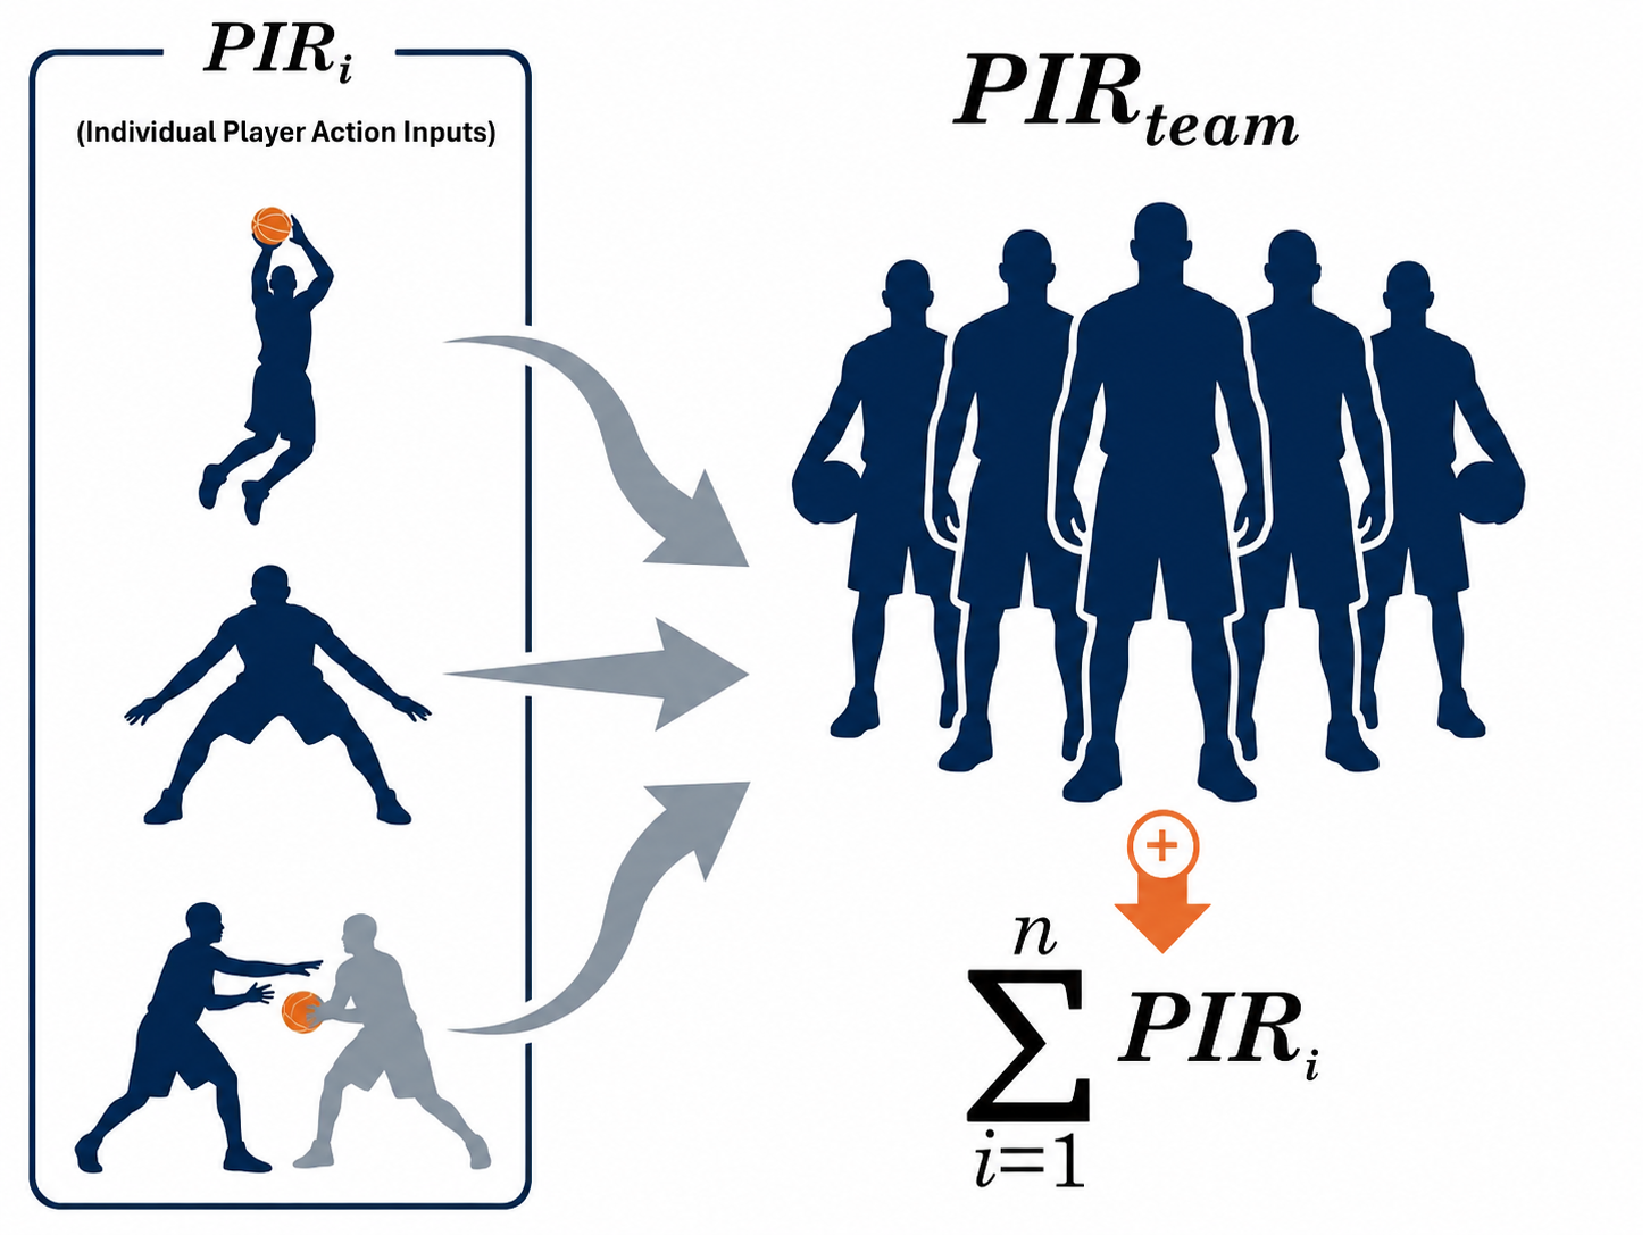
\includegraphics[width=.70\textwidth,trim=10bp 7bp 45bp 7bp,clip]{figures/PIR_team_diagram.pdf}
\caption{Construction of the existing official EuroLeague Performance Index Rating (PIR) at player and team levels. Recorded box-score actions are evaluated under the official PIR formula to obtain each player's \(\mathrm{PIR}_i\). Summation across participating players yields the player-attributed component of official team PIR. The schematic represents official PIR only; it does not depict RM-PIR calibration. Official team rows may additionally include actions that are not allocated to player rows, which are retained through the explicit team-only residual in Equation~\ref{eq:additivity}.}
\label{fig:official-pir-aggregation}
\end{figure}

The ten nonpoint fields were ordered as TR, AST, STL, BLK, FD, MFG, MFT, TO, BLKA and FC. Let \(\mathbf X_{ug}\) contain their unsigned counts and let \(\mathbf s=(1,1,1,1,1,-1,-1,-1,-1,-1)^{\mathsf T}\) contain the official signs. For each completed game, the signed winner--loser design was \(\mathbf x_g=\mathbf s\odot(\mathbf X_{W_g,g}-\mathbf X_{L_g,g})\).

Eight positive raw magnitudes \(\mathbf a\) were estimated. Blocks and blocks against shared one unsigned magnitude, as did fouls drawn and fouls committed; their opposite directions remained encoded by \(\mathbf s\). An expansion matrix \(\mathbf E\in\{0,1\}^{10\times8}\) mapped the eight groups to the ten fields. The fitted nonpoint contrast was \(z_g(\mathbf a)=\mathbf x_g^{\mathsf T}\mathbf E\mathbf a\). For calibration set \(\mathcal A\), transition width \(\tau>0\) and ridge strength \(\alpha>0\), the bounded estimator was
\begin{equation}
\widehat{\mathbf a}_{\mathcal A}(\tau,\alpha)
=\underset{\mathbf a\in[0.5,1.5]^8}{\arg\min}
\left\{
\frac{1}{|\mathcal A|}\sum_{g\in\mathcal A}
\log\!\left[1+\exp\!\left(-\frac{z_g(\mathbf a)}{\tau}\right)\right]
+\frac{\alpha}{10}\left\lVert\mathbf E\mathbf a-\mathbf1_{10}\right\rVert_2^2
\right\}.
\label{eq:objective}
\end{equation}
The first term is a smooth surrogate for nonpoint discordance; the second is a ridge penalty that anchors the ten scored field magnitudes to the official unit convention \cite{hoerl1970}. Points and point margins do not enter Equation~\ref{eq:objective}. The complete derivation, expansion mapping, gradient, strict-convexity argument and numerical checks are given in Supplementary Section S1.

Within each eligible prior-season window, \(\tau\) and \(\alpha\) were selected on a chronological 70/30 split of distinct game dates. The selected specification was refitted on the complete window. The first three target seasons used all available prior seasons, and the final two used the latest three completed seasons. No target-season observation entered selection, refitting or scale matching, following the logic of out-of-time evaluation under possible temporal change \cite{Tashman2000,GamaEtAl2014}. Figure~\ref{fig:workflow} summarises this procedure.

\begin{figure}[t]
\centering
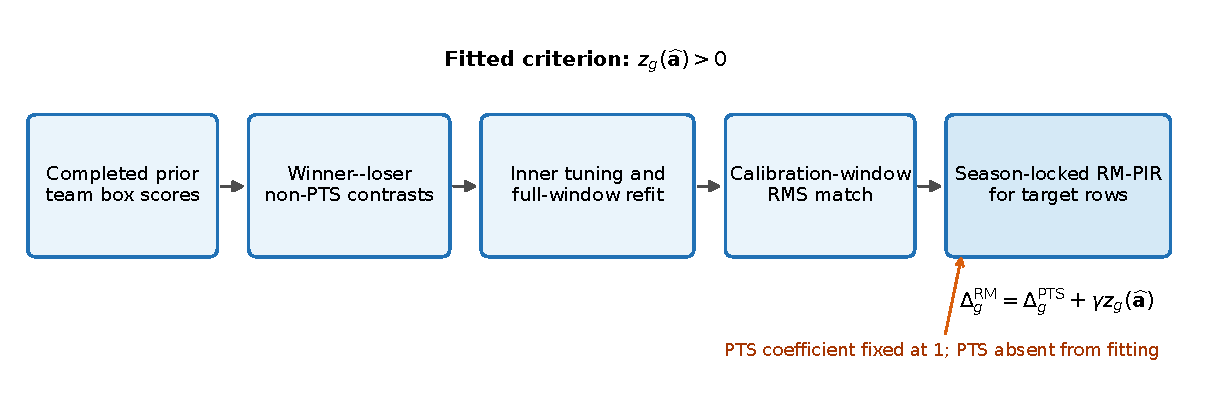
\includegraphics[width=\textwidth]{figures/vppir_methodology.pdf}
\caption{Season-locked RM-PIR procedure. Hyperparameters are selected within the eligible prior-season window, the selected model is refitted on that complete window, and a common RMS factor places the fitted nonpoint contrast on the official calibration-window scale. Points retain coefficient one and are restored only when the complete target-season score is assembled.}
\label{fig:workflow}
\end{figure}

Let \(o_g=\mathbf x_g^{\mathsf T}\mathbf1_{10}\) be the official calibration contrast and \(q_{g,Y}=\mathbf x_g^{\mathsf T}\mathbf E\widehat{\mathbf a}_Y\) the fitted raw contrast for target season \(Y\). The positive scale factor and final signed coefficients were
\begin{equation}
\gamma_Y=
\sqrt{\frac{\sum_{g\in\mathcal C_Y}o_g^2}
{\sum_{g\in\mathcal C_Y}q_{g,Y}^2}},
\qquad
\mathbf c_Y=\gamma_Y\operatorname{diag}(\mathbf s)\mathbf E\widehat{\mathbf a}_Y,
\qquad
\rmpir_{ug}^{(Y)}=\mathrm{PTS}_{ug}+\mathbf X_{ug}^{\mathsf T}\mathbf c_Y.
\label{eq:score}
\end{equation}
Equation~\ref{eq:score} equates the uncentred second moments, or RMS values, of official and fitted nonpoint contrasts within the calibration window. It does not equate centred variances, means, target-season distributions or player-score distributions. Because \(\gamma_Y>0\), it cannot change the sign of a fitted nonpoint contrast. Table~\ref{tab:coefficients} gives the official and locked 2025--26 coefficients.

\begin{table}[t]
\caption{Official PIR coefficients and the RM-PIR coefficients locked for 2025--26. The RM-PIR vector was selected, fitted and RMS-matched using 2022--23 through 2024--25 only. Raw magnitudes were bounded before the common RMS factor was applied; consequently the final coefficient magnitudes need not lie in \([0.5,1.5]\).}
\label{tab:coefficients}
\centering
\small
\begin{tabular}{@{}lrrl@{}}
\toprule
Field & Official PIR & 2025--26 RM-PIR & Interpretation \\
\midrule
PTS  &  1.000 &  1.000 & points \\
TR   &  1.000 &  1.431 & total rebounds \\
AST  &  1.000 &  0.624 & assists \\
STL  &  1.000 &  1.508 & steals \\
BLK  &  1.000 &  0.510 & blocks \\
FD   &  1.000 &  0.510 & fouls drawn \\
MFG  & -1.000 & -1.318 & missed field goals \\
MFT  & -1.000 & -0.997 & missed free throws \\
TO   & -1.000 & -1.531 & turnovers \\
BLKA & -1.000 & -0.510 & blocks against \\
FC   & -1.000 & -0.510 & fouls committed \\
\bottomrule
\end{tabular}
\end{table}

\subsection{Temporal evaluation, uncertainty and robustness}

The rolling targets were 2021--22 through 2025--26. The corresponding calibration windows were 2020--21; 2020--21 to 2021--22; 2020--21 to 2022--23; 2021--22 to 2023--24; and 2022--23 to 2024--25. We reported winner-higher/tie/loser-higher (W/T/L) counts and the signed paired change in the proportion of discordant games. Negative changes favour RM-PIR. Descriptive Wilson intervals were calculated for each score's discordance proportion. Paired differences used 20,000 whole-game bootstrap replicates, and paired transitions were examined with the exact McNemar calculation \cite{wilson1927,mcnemar1947,efron1979,efron1993}. Because games share clubs, the focal season also used a club-membership resampling sensitivity, motivated by multiway resampling for non-independent membership structures \cite{Owen2007}, and a joint procedure that refitted calibration coefficients and resampled target-club membership. These remain descriptive dependence checks rather than a hierarchical generative model.

Sensitivity analyses changed the coefficient bounds, calibration-window length, hyperparameter grid and temporal selection rule; excluded overtime; omitted calibration seasons and target clubs; separated the paired block and foul groups; used pace-normalised contrasts; excluded team-only residuals; restricted evaluation to the regular season; and replaced RMS matching with five alternative scale conventions. Full definitions and results are in Supplementary Sections S4--S5.

\subsection{Additivity and secondary player diagnostics}

The same locked coefficients can be applied to official player rows, but team rows may contain actions not allocated to a player. For component \(j\), define \(r_{tgj}=X_{tgj}-\sum_{i\in t}X_{igj}\) and define the points residual analogously. The exact accounting identity is
\begin{equation}
\rmpir_{tg}^{(Y)}=
\sum_{i\in t}\rmpir_{ig}^{(Y)}+
\left(r_{tg,\mathrm{PTS}}+\sum_{j=1}^{10}c_{j,Y}r_{tgj}\right).
\label{eq:additivity}
\end{equation}
The bracketed term is the explicit team-only residual. Equation~\ref{eq:additivity} establishes algebraic decomposition, not causal attribution.

Player analyses were secondary and exploratory. They included all positive-minute 2025--26 player-games, raw and exposure-adjusted Spearman association with official on-court plus-minus, and association with plus-minus in the next one or three appearances. These diagnostics were used to delimit interpretation, not to select coefficients or claim individual-level validity. Complete player rankings and definitions are supplied in Supplementary Section S6 and in the machine-readable supplementary table.

\section{Results}

\subsection{Sample and data integrity}

The analysis contained 2,018 completed games (4,036 team-game rows): 328, 299, 328, 331, 330 and 402 games from 2020--21 through 2025--26, respectively. The five out-of-time target seasons contained 1,690 games. Every official team PIR value was reconstructed exactly, no required primary field was missing, no negative attempts-minus-makes value remained and no target observation entered its calibration window.

\subsection{Primary complete-score result and nonpoint mechanism}

In 2025--26, official complete PIR produced 375 winner-higher, 3 tied and 24 loser-higher games; RM-PIR produced 381, 0 and 21. Discordances decreased from 27/402 (6.72\%) to 21/402 (5.22\%), a paired change of -1.49 percentage points (game-bootstrap 95\% interval, -3.23 to 0.25). RM-PIR reclassified nine official discordances into concordance and introduced three new discordances. With a common 0.5-PIR-unit equivalence band, the net strict gain decreased from six to three games. Figure~\ref{fig:changed} shows the observed complete-score transitions.

\begin{figure}[t]
\centering
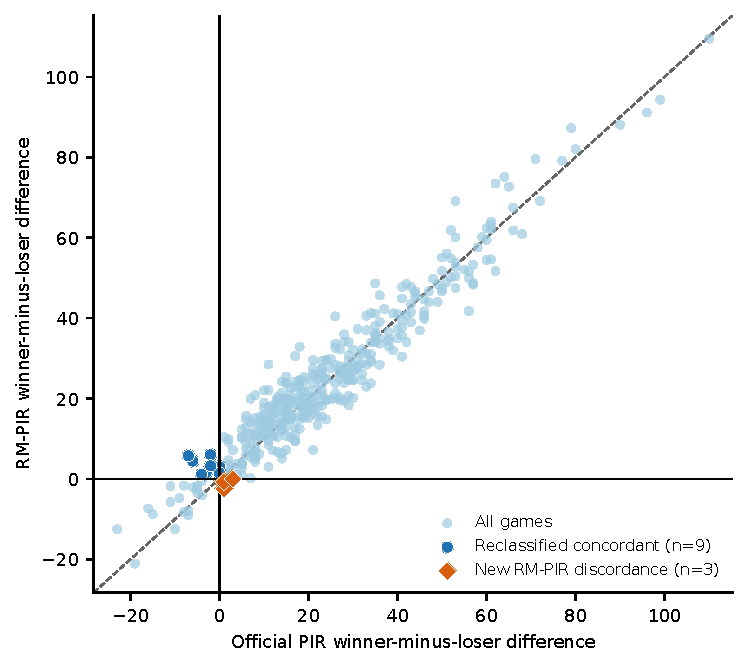
\includegraphics[width=\textwidth]{figures/vppir_changed_games.pdf}
\caption{Complete-score winner--loser contrasts in the 402 games of 2025--26. Grey points are concordant under both scores, blue points are games reclassified into concordance by RM-PIR, and orange diamonds are newly discordant games. The horizontal and vertical zero lines mark the strict ordering boundary.}
\label{fig:changed}
\end{figure}

The nonpoint result was larger and more stable. Official nonpoint PIR produced W/T/L counts of 334/14/54, compared with 357/0/45 for RM-PIR. Discordances decreased from 68 (16.92\%) to 45 (11.19\%), a paired change of -5.72 percentage points (game-bootstrap 95\% interval, -8.46 to -2.99). Twenty-eight games moved into concordance and five became newly discordant. The club-membership interval was -11.14 to -0.84 percentage points, and the joint coefficient-refit/club-membership interval was -11.48 to -1.90. As expected from the positive scale factor, all six scale conventions gave the same 357 nonpoint winner-higher games.

\subsection{Rolling historical backtests}

Complete-score discordance decreased in every target season (Table~\ref{tab:rolling}). Pooled descriptively across 1,690 target games, discordances decreased from 150 under official PIR to 104 under RM-PIR (-2.72 percentage points); 54 games moved into concordance and eight became newly discordant. Nonpoint discordances decreased from 293 to 209 (-4.97 percentage points), with a negative season-specific change in all five targets. Figure~\ref{fig:rolling} displays the target-season paths. Pooled values are descriptive summaries rather than an additional independently designed test.

\begin{table}[t]
\caption{Rolling historical backtests. W/T/L denotes winner higher/tie/loser higher. The signed change is the RM-PIR discordance percentage minus the official PIR discordance percentage; negative values favour RM-PIR. Intervals are paired whole-game bootstrap 95\% intervals.}
\label{tab:rolling}
\centering
\tiny
\setlength{\tabcolsep}{1.5pt}
\begin{tabular}{@{}llrccrrc@{}}
\toprule
Target & Score & Games & Official W/T/L & RM-PIR W/T/L & Change (pp) & 95\% interval & Corrected/new \\
\midrule
2021--22 & Nonpoint & 299 & 251/3/45  & 267/0/32 & -5.35 & [-8.36, -2.34] & 19/3 \\
         & Complete &     & 273/4/22  & 282/0/17 & -3.01 & [-5.02, -1.34] & 9/0 \\
2022--23 & Nonpoint & 328 & 272/4/52  & 284/0/44 & -3.66 & [-6.40, -1.22] & 16/4 \\
         & Complete &     & 294/5/29  & 304/0/24 & -3.05 & [-5.18, -0.91] & 12/2 \\
2023--24 & Nonpoint & 331 & 274/12/45 & 289/0/42 & -4.53 & [-7.55, -1.81] & 19/4 \\
         & Complete &     & 300/2/29  & 307/0/24 & -2.11 & [-4.23, -0.30] & 9/2 \\
2024--25 & Nonpoint & 330 & 266/6/58  & 284/0/46 & -5.45 & [-8.48, -2.73] & 22/4 \\
         & Complete &     & 298/3/29  & 312/0/18 & -4.24 & [-6.67, -2.12] & 15/1 \\
2025--26 & Nonpoint & 402 & 334/14/54 & 357/0/45 & -5.72 & [-8.46, -2.99] & 28/5 \\
         & Complete &     & 375/3/24  & 381/0/21 & -1.49 & [-3.23, 0.25]  & 9/3 \\
\bottomrule
\end{tabular}
\end{table}

\begin{figure}[t]
\centering
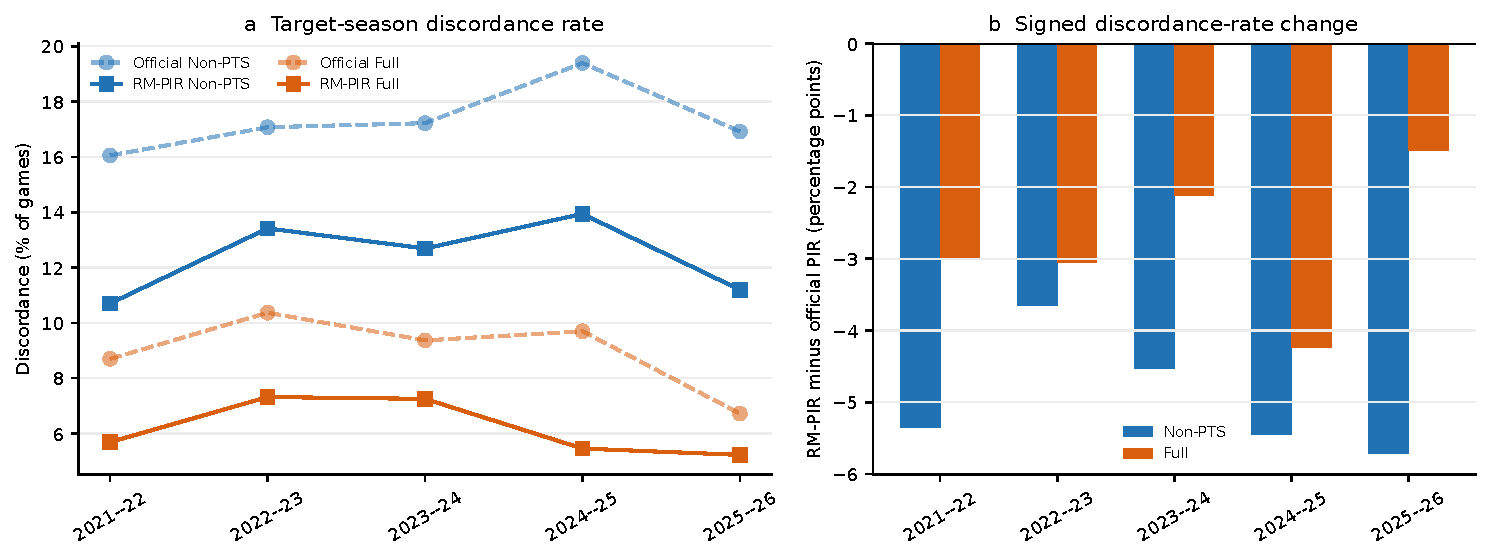
\includegraphics[width=\textwidth]{figures/vppir_historical_validation.pdf}
\caption{Rolling historical target-season results. The upper panels show discordance rates for official PIR and locked RM-PIR; the lower panels show the signed RM-PIR minus official change. Complete scores are the primary operational outcome and nonpoint scores are the mechanism analysis.}
\label{fig:rolling}
\end{figure}

\subsection{Coefficient stability and robustness}

For 2025--26, inner selection chose \(\tau=5\) and \(\alpha=0.01\); the complete-window scale factor was \(\gamma=1.0205\). The final nonpoint magnitudes ranged from 0.510 to 1.531 (Table~\ref{tab:coefficients}). Turnovers reached the upper raw bound, whereas blocks/blocks against and fouls drawn/committed reached the lower raw bound. Boundary activity means that these estimates are partly determined by the stated feasible region and should not be interpreted as unconstrained action values.

Coefficient paths varied across targets, especially for rebounds, steals, missed shots and turnovers (Figure~\ref{fig:coefficients}). Nevertheless, all final fits converged, the largest analytic-versus-numerical gradient discrepancy was \(8.91\times10^{-9}\), dispersed-start solutions agreed within \(5.06\times10^{-7}\), and the maximum RMS identity error was \(3.55\times10^{-15}\). Across the prespecified and retrospective 2025--26 sensitivities, every nonpoint discordance change remained negative. Complete-score changes were smaller and more scale-dependent, consistent with restoration of the fixed point margin after nonpoint fitting.

\begin{figure}[t]
\centering
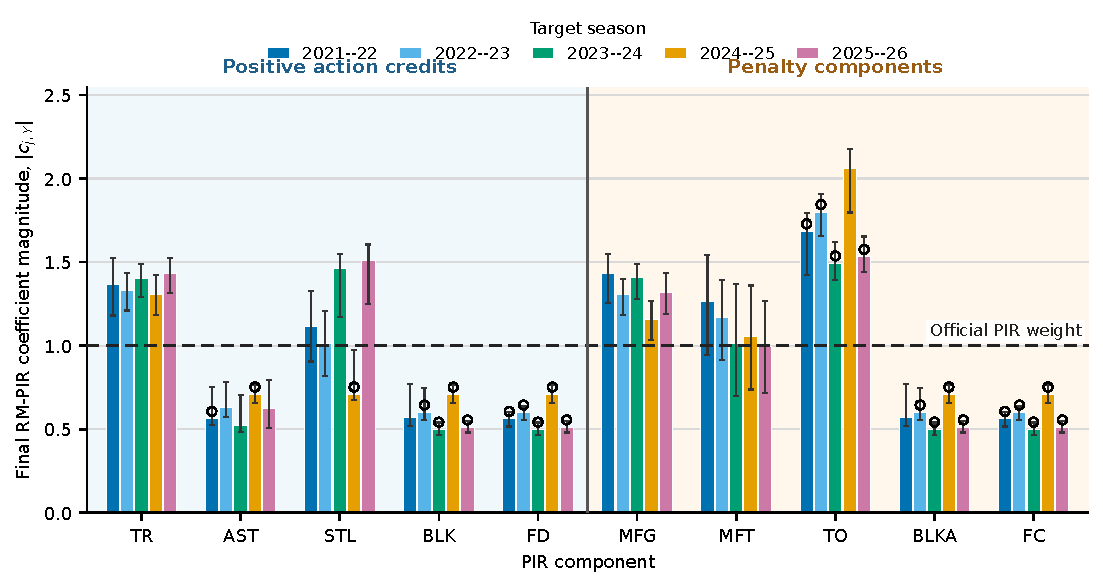
\includegraphics[width=\textwidth]{figures/vppir_coefficient_stability.pdf}
\caption{Locked RM-PIR coefficient magnitudes across target seasons. Credits are shown to the left of the separator and penalties as absolute magnitudes to the right. The dashed line is the official unit magnitude. Open markers identify coefficients whose raw magnitude was on a bound before RMS matching.}
\label{fig:coefficients}
\end{figure}

\subsection{Team additivity and secondary player findings}

The component-wise residual identity held to numerical precision in all evaluated seasons (Table~\ref{tab:audits}). The points residual was zero in every team-game; other team-only actions were retained explicitly rather than assigned to individual players. In the equal-exposure 2025--26 regular season, the top four teams by PIR remained the top four under RM-PIR. Dubai had the largest upward movement (ninth to sixth), while Maccabi had the largest downward movement (fifth to seventh). Complete regular-season and all-stage team rankings are reported in Supplementary Tables S5--S6.

Player-level findings did not support a validation claim. Across 8,741 positive-minute player-games, raw Spearman association with on-court plus-minus was 0.301 for official PIR and 0.319 for RM-PIR. After rank-based adjustment for estimated possession exposure, the correlations were 0.280 and 0.294. Associations with the next appearance or the next three appearances were close to zero and slightly lower for RM-PIR than for official PIR. The team-fitted weights therefore remain an algebraically applicable player score, not an established individual-impact measure.

\begin{table}[t]
\caption{Arithmetic, team and exploratory player audit summary. Player associations are descriptive Spearman correlations and were not used for coefficient selection.}
\label{tab:audits}
\centering
\small
\begin{tabular}{@{}p{0.48\textwidth}rr@{}}
\toprule
Audit & Official PIR & RM-PIR \\
\midrule
Exact team-score reconstructions, all seasons & 4,036/4,036 & 4,036/4,036 \\
Maximum absolute additivity-identity error & 0 & \(4.22\times10^{-14}\) \\
2025--26 regular-season team rank: Dubai & 9 & 6 \\
2025--26 regular-season team rank: Maccabi & 5 & 7 \\
Player-game correlation with on-court plus-minus & 0.301 & 0.319 \\
Exposure-adjusted player-game correlation & 0.280 & 0.294 \\
Correlation with next-appearance outcome & 0.0228 & 0.0195 \\
Correlation with next-three-appearance outcome & 0.0347 & 0.0300 \\
\bottomrule
\end{tabular}
\end{table}

\section{Discussion}

RM-PIR improved the concordance of the EuroLeague team action ledger with completed-game outcomes in each of five rolling historical target seasons. The nonpoint result was larger and more consistent than the complete-score result, which is the expected pattern when weights are learned without points and the fixed point margin is then restored. In the latest season, the complete-score interval included no difference, whereas nonpoint improvements persisted under game, club-membership and joint coefficient/club resampling. The evidence is therefore strongest for the fitted action direction and more limited for the downstream complete score.

The contribution is methodological rather than a new theory of basketball value. Existing EuroLeague studies identify associations between particular box-score actions and winning, qualification or season success \cite{Ozmen2016,Cene2018,MikolajecEtAl2021,KamitsisPolitis2025}. RM-PIR instead asks whether those heterogeneous actions can be reweighted while preserving the official ledger's transparency, point coefficient and approximate contrast scale. Unlike possession, lineup, adjusted plus-minus or tracking models, it requires no unobserved contextual data and introduces no player-specific parameter \cite{Oliver2004,CharamisEtAl2023,DeshpandeJensen2016,GhimireEtAl2020}. That simplicity is useful for auditability but necessarily limits interpretation.

Several qualifications are central. First, winner-higher ordering is an author-selected criterion, and the complete score is mechanically related to the game result through points. Second, the model class, restrictions and evaluation plan were developed after historical seasons had been inspected; temporal exclusion prevents direct leakage into each target fit but does not make the analysis preregistered or prospective. Third, archived bylaws document earlier statistical governance but not exact stability of every scoring definition. Fourth, several raw coefficients were boundary-active, and complete-score performance was sensitive to scale choice. Fifth, recurring teams and schedules limit independence; resampling analyses describe robustness but do not replace a hierarchical competition model. Finally, a box-score ledger omits important contextual contributions, and the exploratory player diagnostics showed little next-appearance association. RM-PIR should not be described as adjusted plus-minus, causal player impact, predictive player value or a complete performance measure.

A prospective study should freeze the action groups, bounds, hyperparameter rule and RMS anchor before a future season, archive the applicable scoring manual and raw extraction date, and evaluate the locked score without further design changes. If an official event-definition change is documented, the calibration window should restart. Player-level development would require a distinct estimand and richer possession, lineup and tracking data rather than inference from team-ledger concordance alone.

\section{Data availability}

The source team and player box scores are publicly accessible through Euroleague Basketball's statistics service, and game records through its Game Center \cite{euroleagueStats,EuroleagueGameCenter2026}. Subject to provider terms, the analysis-ready dataset, exclusion register, machine-readable supplementary tables and metadata will be deposited in a persistent repository. [Repository name, DOI, licence and access conditions.]

\section{Code availability}

The complete analysis code, locked environment specification and deterministic audit outputs are prepared for archival release. [Persistent repository identifier, licence and access conditions.]

\section{Acknowledgements}

[Acknowledgements and verified funding information.]

\section{Author contributions}

[Author contributions, identified by initials in accordance with the journal's authorship policy.]

\section{Funding}

[Verified funding statement.]

\section{Competing interests}

[Competing-interests declaration.]

\section{Generative AI use}

During manuscript preparation, the authors used OpenAI Codex for language editing, source-code review and reproducibility checks. The authors reviewed and verified all resulting text, calculations and references and take full responsibility for the manuscript.

\section{Additional information}

Supplementary Information accompanies this manuscript. Correspondence and requests for materials should be addressed to [corresponding author and contact details].

\bibliography{bibliography}

\end{document}
